\documentclass[fleqn]{jaes}

% Metadata Information
\jyear{2025}
\jmonth{October}

\usepackage{amsmath}\setlength{\mathindent}{10pt}
\usepackage{bm}
% Use standard mathcal instead of pazocal to avoid font issues
\newcommand{\pazocal}{\mathcal}


\begin{document}

% Page heads
\markboth{AHONIEMI, MONTENEZ AND STENQVIST}{MODELING UNDERWATER SOUND PROPAGATION}


% Title portion
\title{Modeling underwater sound propagation}

%Author Info.
\authorgroup{
\author{OTTO AHONIEMI}, \author{HOCINE MONTENEZ}
AND \author{ATTE STENQVIST}
}

%Abstract
%An informative and self-contained abstract of 100 to 200 words must be provided. The abstract should mention the motivation, problem statement, approach, results, and implications of the work, usually with one or two sentences each. It is recommended that the abstract be written in a single paragraph without citing any references. The Journal of the Audio Engineering Society is a modern scientific journal supporting online publishing with colors and a graphical abstract. It is a hybrid journal publishing both Open Access and traditional papers, the latter being only available for subscribers, such as AES members. If a paper published in the Journal of the Audio Engineering Society has been made Open Access, it will have the OA logo next to it and will be freely downloadable from the AES E-Library by anyone, even if they are not an AES member or E-Library subscriber. This example abstract contains 149 words.
\abstract{%
}
\maketitle
%Head 1
% \section{INTRODUCTION}
% \subsection{Context}
% %What why
% %Why its more difficult than we expect snell, ssp, etc


% \subsection{Literature review}
% \begin{itemize}
%     \item SSP equation more precise/different conditions Atte 
%     \item Ray reflection on the seabed H
%     \item Transfer loss H
%     \item Impact of ray propagation on animals? Otto
%     \item Impact of fish on propagation? Otto
% \end{itemize}

% \begin{itemize}
%     \item ray based methods H
%     \item other blablabla based methods Otto
% \end{itemize}


% \section{METHODS="models"}
% \subsection{Dumb euler}

% \subsection{C-linear}
% \subsection{BellHop}

% \newpage
% \clearpage
\section{INTRODUCTION}

\subsection{Sound propagation in the ocean}
In ocean acoustics, sound is propagated using the ocean as a waveguide, limited between the surface and the seafloor. Within this waveguide, speed of sound varies due to density, which in the ocean is related to static pressure, salinity and temperature. Many different empirical formulas for calculating the speed of sound have been proposed \cite{Huang} with varying complexities and application ranges, but for most cases the simplified Medwin empirical formula can be used as a an approximation \cite{Jensen}, \cite{Lurton}. In the Medwin formula, speed of sound ($c$, in $m/s$) is calculated as 

\begin{equation}
\begin{split}
c &= 1449.2 + 4.6T - 0.055T^2 + 0.00029T^3 \\
  &\quad + (1.34 - 0.01T)(S-35) + 0.016z
\end{split}
\label{eq:speedofsound}
\end{equation}
where $T$ is the temperature, in °C; $S$ is the salinity and $z$ is the depth, in $m$. 

Due to the variety of temperature, salinity and depth in the oceans around the world, underwater sound propagation is strictly dependent on the \textit{sound speed profile} (SSP) that is used. A typical SSP in deep non-polar oceans has an unstable mixed layer near the surface and a stable, linearly increasing sound speed profile in the deep isothermal layer near the seafloor \cite{Jensen}. Between these regions exists the \textit{deep sound channel}, where the speed of sound reaches a minimum. The \textit{Munk profile}, is an idealized SSP showcased in Fig. \ref{fig:munk}, which contains many features of deep-water propagation and is often used for demonstrations of deep-water propagation.

For determining the sound propagation paths, speed of sound is treated in the same way the index of refraction is treated in optics. The refraction of the propagation direction changes as the speed of sound changes in accordance with \textit{Snell's law}, 

\begin{equation}
\frac{\cos{\theta}}{c}= p,
\label{eq:snellslaw}
\end{equation}

where $p$ is a constant, $\theta$ is the ray angle and $c$ is the local speed of sound \cite{Lurton}. Sound rays will therefore bend towards regions with lower speed of sound. A demonstration of deep-water propagation paths using the Munk profile is shown in Fig \ref{fig:munk}.

\begin{figure*}
\centering
\centering
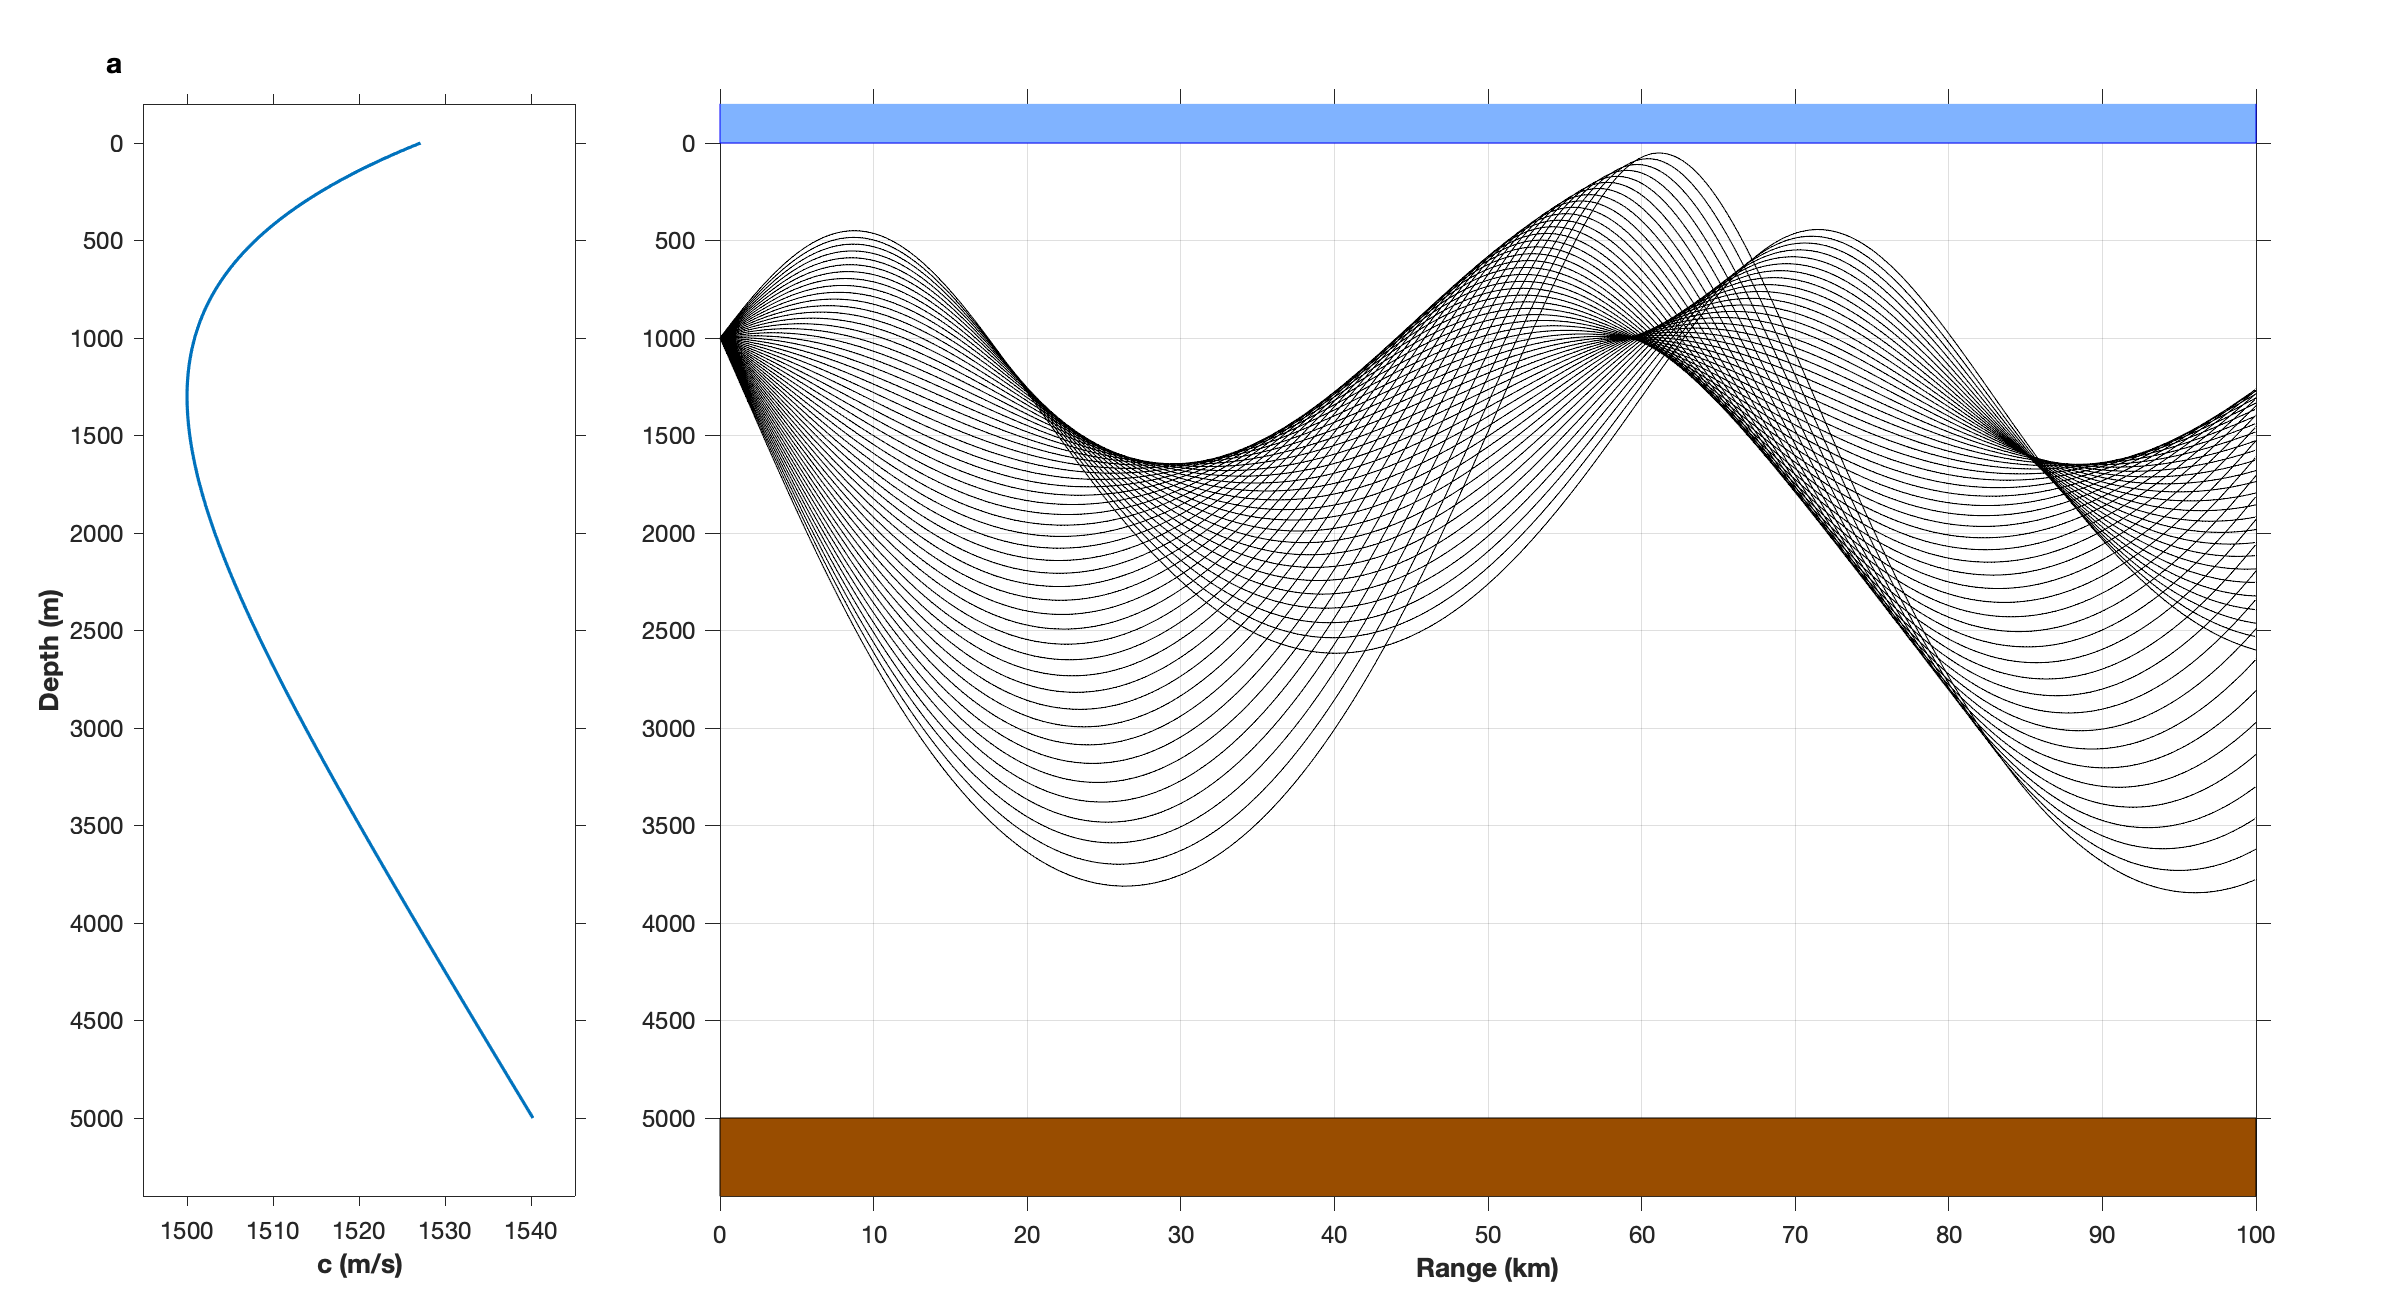
\includegraphics[trim=0cm 0.5cm 0cm 0.5cm, width=0.8\textwidth]{sspExample.png}
\caption{Munk sound speed profile (left) and sound propagation rays in Munk sound speed profile (right). Ray tracing using C-linear method.}
\label{fig:munk}
\end{figure*}

\subsection{Reflections}
At the surface and at the seabed of the ocean, the waves will experience reflections. In general, when the medium is not perfectly lossless, the local sound speed $c$ becomes complex, and the reflection coefficient is therefore also complex. Each reflection introduces both an amplitude loss and a phase shift. The reflection coefficient $\pazocal{R}$ and transmission coefficient $\pazocal{T}$ at an interface between two fluid media can be expressed in terms of their specific acoustic impedances $\pazocal{Z}_i = \rho_i c_i / \sin\theta_i$ as

\begin{equation}
\pazocal{R} = \frac{\pazocal{Z}_2 - \pazocal{Z}_1}{\pazocal{Z}_2 + \pazocal{Z}_1}
\quad\quad
\pazocal{T} = \frac{2\pazocal{Z}_2}{\pazocal{Z}_2 + \pazocal{Z}_1}.
\end{equation}

When the two media have similar acoustic impedance ($\pazocal{Z}_1 \approx \pazocal{Z}_2$), the reflection coefficient is almost zero. Conversely, when medium 2 has a much larger impedance than medium 1, the reflection coefficient is close to 1, meaning that most of the energy is reflected.

\subsubsection{Surface reflections}
At the interface, the difference in acoustic impedance between air and water is so large that almost total reflection occurs ($\pazocal{R} \approx 1$). The surface can therefore be approximated as a perfectly reflecting boundary. However, this assumption breaks down in agitated conditions when wind and waves generate bubbles that scatter and absorb acoustic energy, leading to non negligible reflection losses \cite{Jensen}. 

In deep water, this bending traps the acoustic energy, hence creating ray paths that travel long distances without ever touching the bottom and that only reflect from the surface. Such typical deep-water environments, where these effects are prominent, occur in all oceans at depths exceeding about 2000m \cite{Jensen}. In this case, sound propagation often occurs without significant bottom interaction, dominated instead by refraction and surface reflection.

\subsubsection{Bottom reflections}

Reflection from the ocean bottom is far more complex. Unlike the nearly perfect surface, the bottom is generally a lossy boundary composed of sediments and rock layers with variable density, sound speed, and attenuation. The impedance mismatch between water and seabed materials determines how much energy is reflected versus transmitted into the sediment.

Layered sediments further complicate this behavior, producing frequency- and angle-dependent reflection losses due to interference within the layers. Depending on the incident angle, thin or half-wavelength layers can be acoustically transparent, while quarter-wavelength layers can act as anti-reflecting coatings \cite{Jensen}.

\subsection{Transfer loss}
As waves travel through the water, their amplitude is progressively attenuated by two important effects: absorption and scattering. This attenuation is usually modeled by an exponential decay law with distance $x$:
\begin{equation}
    A = A_0 \exp (-\alpha x)
    \label{eq:attenuationdecay}
\end{equation}
where $A_0$ is the rms amplitude at $x=0$ and $\alpha$ is the attenuation factor.
The coefficient $\alpha$ has some dependence on frequency, temperature, pressure, salinity, and acidity. However, a simplified expression depending only on frequency is considered sufficiently accurate for most problems in ocean acoustics \cite{Jensen, urick1979}: 
\begin{equation}
    \alpha = \frac{1}{8.69} \big[ 3.3 \cdot 10^{-3} + \frac{0.11f^2}{1+f^2} + \frac{44f^2}{4100+f^2} + 3\cdot 10^{-4} f^2\big]
    \label{eq:attenuationfrequency}
\end{equation}
where $f$ is expressed in kHz and $\alpha$ in dB/km. Equation \ref{eq:attenuationfrequency} shows attenuation increases with frequency, such that low-frequency waves are only mildly attenuated, making them highly effective for long-range underwater communication compared to electromagnetic waves. For example, a 100Hz acoustic signal would need to travel around 2200 km to be attenuated by -10dB.

\subsection{Volume scattering (fish)}

In addition to boundary interactions at the sea surface and seafloor, sound propagation in the ocean is affected by volume scattering from marine life within the water column. Volume scattering is characterized by a scattering cross section, defined as the ratio of scattered power to incident intensity on a unit volume. This scattering contributes to both attenuation of coherent acoustic signals and generation of reverberation that interferes with sonar detection.

At lower frequencies (below 10 kHz), fish with gas-filled swim bladders are the dominant volume scatterers \cite{Jensen}. The swim bladder presents a high acoustic impedance contrast with the surrounding tissue and seawater, causing strong backscattering. Above 20 kHz, smaller organisms such as zooplankton become the primary scatterers. The target strength of individual fish depends on fish size, swim bladder morphology, frequency, and orientation relative to the acoustic beam, with typical values ranging from $-$40 to $-$20 dB for individual fish at moderate frequencies \cite{Foote1980}. The swim bladder contribution accounts for 90-95\% of the backscattered energy.

Volume scattering strength generally decreases with depth, with a notable exception being the deep scattering layer (DSL). The DSL is a concentrated layer of marine organisms, primarily small fish and zooplankton, that migrate vertically in the water column following the diurnal cycle. This layer can produce scattering returns comparable in magnitude to those from physical boundaries \cite{Jensen}.

In acoustic propagation modeling, volume scattering introduces two main effects: attenuation of the coherent field through scattering loss, and generation of a diffuse reverberation field. The volume scattering strength $S_v$ is expressed in decibels and relates the scattered intensity to incident intensity per unit volume. For a layer of thickness $H$, the integrated column scattering strength $S_c$ can be computed by integrating the local volume scattering strength $s_v(z)$ over depth. These parameters are used in sonar performance prediction and acoustic propagation models for applications such as fisheries acoustics and marine mammal protection.

\subsection{Sound propagation models}
Underwater sound propagation can be described using several types of models, each based on different approximations of the acoustic wave equation. These models vary in their physical assumptions, numerical complexity, and suitability for particular frequency ranges or environmental conditions. This section briefly presents the most popular families of methods \cite{propagationmodels, Jensen}.

First, ray theory based models describe sound as energy traveling along discrete geometric paths, or rays. This approach is particularly effective when the acoustic wavelength is small compared to the scale of environmental variations, such as at high frequencies or over long distances. The use of ray-based models in the research community was motivated by their simplicity and computational efficiency. However, they neglect diffraction and interference effects, making them less commonly used when it comes to model low frequency phenomena \cite{hovem2019}.

Next, the wave equation can be solved using the separation of variables technique to isolate the vertical and horizontal directions. The vertical wave equation solutions are normal modes, or eigenvalues, that can be summed at the source and receiver to generate the full acoustic field, depending on the horizontal propagation.
Each mode behaves like a standing wave in depth and propagates horizontally with its own phase speed. This approach is particularly suited for low-frequency and long-range propagation, as it can accurately describe the interference patterns between modes. The main drawback of normal mode models is that they become too computationally expensive at high frequencies \cite{propagationmodels}.

Finally, as most of the problems solved in ocean acoustics involve a one-way propagation (i.e. from source to receiver) separating the wave equation into incoming and outgoing solutions leads to the
Parabolic Equation (PE) method. PE models can account for refraction, diffraction, and scattering, which explains why they are so widely used and popular in the research community \cite{Jensen}. The PE computational load increases with the square of the frequency, which generally limits its use to frequencies less than 1 kHz \cite{propagationmodels}.

In summary, each category of sound propagation model offers a different balance between accuracy, complexity and computational cost. The choice of the model is determined by the problem requirements.

\section{METHODS}
Three different underwater sound propagation models are compared in this work. The models \textit{Geometric ray tracing} (described in Section 2.1) and \textit{c-linear} (described in Section 2.2) are simple ray-based methods based on techniques represented in \cite{Jensen}. The \textit{Bellhop} model described in Section 2.3 is a more advanced beam tracing program using open source code from \cite{Porter}.

\subsection{Geometric Ray Tracing}
The underwater acoustic propagation is first modeled using geometric ray tracing, governed by Snell's law. This simple method does not solve the full acoustic wave equation, but approximates the trajectories of sound waves as they travel through the horizontally stratified water environment. 

The environment is represented by a one-dimensional sound speed profile $c(z)$ that varies with depth $z$.
A simple Munk-like profile \cite{Porter} is employed to approximate realistic ocean conditions:
\begin{equation}
    c(z) = c_0 \left[ 1 + \epsilon \left( \bar{z} - 1 + e^{-\bar{z}} \right) \right],
    \quad \text{where} \quad
    \bar{z} = \frac{2(z - z_0)}{z_0}.
\end{equation}
where $c_0 = 1500~\text{m/s}$ is the reference sound speed, $z_0 = 1300~\text{m}$ is the reference depth (the sound channel axis), and $\epsilon = 0.00737$ is a non-dimensional perturbation parameter controlling the strength of the sound speed variation. 

The trajectory of the ray is governed by the differential equations:
\begin{equation}
    \frac{dx}{ds} = \cos\theta \quad \quad
    \frac{dz}{ds} = \sin\theta,
    \label{eq: dsRelations}
\end{equation}
where $s$ is the arclength along the ray. The local angle $\theta$ can be recovered from Snell’s law:
\begin{equation}
    \theta(z) = \arccos\!\left(p\,c(z)\right),
\label{eq:arccosSnell}
\end{equation}
provided that $|p\,c(z)| \leq 1$, where $p$ is the Snell's law constant.

\subsubsection{Numerical Integration}

The ray paths were computed by discretizing the arclength $s$ into small steps of size $\Delta s$ and updating the horizontal and vertical positions as
\begin{align}
    x_{n+1} &= x_n + \Delta s \cos\theta_n, \\
    z_{n+1} &= z_n + \Delta s \sin\theta_n,
\end{align}
where $\theta_n$ is evaluated at the current depth using Snell’s law. 

At each step, reflections from the sea surface and bottom boundaries were handled by reversing the vertical direction of propagation:
\begin{equation}
    \sin\theta_{n+1} = -\,\sin\theta_n,
    \label{Perfectreflection}
\end{equation}
whenever the ray reached $z = 0$ (surface) or $z = z_{\text{max}}$ (bottom).

\subsubsection{Source and Receiver Configuration}

A point source was positioned at depth $z_s = 1000~\text{m}$, and multiple rays were launched at different initial grazing angles $\theta_0$ spanning from $-25^\circ$ to $5^\circ$. 
Each ray was propagated through the water medium until it reached the maximum range or depth limits. 
A receiver was placed at $z_r = 1000~\text{m}$ and $x_r = 100~\text{km}$. 
Rays whose terminal positions fell within a prescribed tolerance of the receiver depth were identified as eigenrays connecting the source and receiver.

\subsection{Cell method: \textit{c}-linear}
Cell methods refer to the practice of calculating rays by dividing the medium into smaller discretized elements with simple properties. This can be done for range-dependent mediums by dividing the medium into triangles \cite{Jensen}. A simple implementation of the cell method \textit{c}-linear in a range-independent medium is presented. 

\subsubsection{Ray tracing using \textit{c}-linear}
Assuming linear sound speed within a discretized step, the \textit{c}-linear method can be used for calculating ray tracing \cite{Jensen}. Compared to the method of geometric ray tracing described in Section 2.1, which interpolates the ray at a discretized step as a straight line from start to end, \textit{c}-linear calculates the step as a circular arc based on the linear variation in depth $g$ from the sound speed

\begin{equation}
c(z) = c_0+gz,
\label{eq:linearSpeed}
\end{equation}

where $c_0$ is the initial sound speed at the start of a step and $z$ is the depth. 

From the local angle in Snell's law derived in Eq. \ref{eq:arccosSnell}, the change in angle over the ray path can further be derived as
\begin{equation}
    \frac{d\theta}{ds}= -\frac{p}{\sin\theta}\frac{dc}{ds} = -\frac{p}{\sin\theta}\frac{\delta c}{\delta z} \frac{dz}{ds}.
\end{equation}

Since it is assumed that the change of speed of sound over depth is constant, and using relations in Eq. \ref{eq: dsRelations} the last two terms can be substituted as

\begin{equation}
    \frac{d\theta}{ds} = -\frac{p}{\sin\theta}g \sin\theta = -gp,
\end{equation}
which is a constant. A constant ray curvature $d\theta/ds$ signifies that the ray follows the path of a circular arc. The angle of the ray at the end of the step is
\begin{equation}
    \theta_{n+1}=\theta_n+\frac{d\theta}{ds}ds=\theta_n-gp \cdot ds,
\end{equation}
where $ds$ is the step length and $n$ is an arbitrary discretized step.

\subsubsection{Implementation}
The \textit{c}-linear method is implemented as an alternative algorithm for calculating ray tracing within a discretized step in an otherwise similar implementation as in Section 2.1 using the same discretization step length, environment, eigenray calculation, and source and receiver configuration. To calculate reflections, a boundary hit point within the step is calculated using linear interpolation if $z\geq z_{max}$ or $z\leq z_{min}$ and specular reflection is assumed as in Eq. \ref{Perfectreflection}.

\subsection{Bellhop}

Bellhop is a beam tracing program developed by Michael Porter as part of the Acoustics Toolbox \cite{Porter}. Unlike simple ray-based methods that treat acoustic paths as infinitesimally thin lines, Bellhop employs Gaussian beam tracing, where each ray has a finite width. This approach can reduce artifacts near caustics and boundaries that are problematic for pure ray methods.

The Gaussian beam formulation extends traditional ray theory by associating a complex beam width parameter with each ray. As the beam propagates through the medium, both its center trajectory and width evolve according to coupled differential equations. For a beam with width parameter $q(s)$, the evolution along arc length $s$ is governed by

\begin{equation}
\frac{dq}{ds} = \frac{c^2}{q} \nabla^2 c,
\end{equation}

where $c$ is the local speed of sound and $\nabla^2 c$ represents the second derivative of the sound speed profile. This formulation allows handling of regions where rays converge (caustics) without the singularities that occur in pure ray methods. At each receiver location, contributions from all beams are summed with appropriate amplitude and phase corrections based on beam geometry.

Bellhop's numerical integration uses an adaptive step size algorithm that automatically adjusts to ensure ray paths accurately land on discontinuities in the sound speed profile, such as at SSP points and boundary segments. This approach ensures proper handling of refraction at layer interfaces and specular reflections at boundaries. The integrator follows the standard ray equations derived from Snell's law in stratified media, with additional terms to track beam spreading and curvature.

\subsubsection{Configuration via .env Files}

Bellhop reads its environmental parameters from text files with the `.env` extension, following a standardized format used throughout the Acoustics Toolbox. These files specify the complete acoustic environment including the sound speed profile, boundary conditions, source and receiver positions, and computational parameters.

The boundary specification allows three main types: Vacuum boundaries (`V`) produce perfect reflection with no transmission; Rigid boundaries (`R`) enforce zero normal particle velocity; and Acoustic halfspace boundaries (`A`) model the seabed as a fluid halfspace with specified sound speed, density, and attenuation. For the acoustic halfspace option, parameters are given as depth, sound speed, shear speed (zero for fluid), density, compressional attenuation, and shear attenuation. These boundary models range from simple geometric reflection to frequency-dependent bottom interaction.

Bellhop supports multiple run types specified in the `.env` file: Ray tracing (`R`) outputs the full geometric paths of all launched rays; Eigenray (`E`) identifies only those rays connecting source to receiver; Coherent transmission loss (`C`) computes the complex pressure field by summing beam contributions with phase information; Incoherent transmission loss (`I`) sums intensities without phase; and Semicoherent (`S`) uses a hybrid approach. The choice of run type will determine both the computational cost and the physical interpretation of results.

\subsubsection{Coherent and Incoherent Summation}

Bellhop can perform both coherent and incoherent field summation. In coherent mode (`C`), the complex acoustic pressure at each receiver is computed by summing contributions from all beams with their relative phases preserved:

\begin{equation}
p(\mathbf{r}) = \sum_{j=1}^{N} A_j e^{i\phi_j},
\end{equation}

where $A_j$ and $\phi_j$ are the amplitude and phase of the $j$-th beam contribution, and $N$ is the total number of beams reaching the receiver. This will produce interference patterns including constructive and destructive interference, which are physically realistic for coherent sources and receivers at fixed positions.

In incoherent mode (`I`), only intensities are summed, discarding phase information:

\begin{equation}
I(\mathbf{r}) = \sum_{j=1}^{N} |A_j|^2.
\end{equation}

This approach is appropriate when modeling averaged fields over many source or receiver positions, or when the acoustic field has significant temporal or spatial incoherence. Incoherent summation produces smoother transmission loss patterns without the fine interference structure of coherent calculations. The simple ray-based methods presented in earlier subsections implicitly perform an operation similar to incoherent summation by counting ray arrivals without tracking phase.

\section{RESULTS}

\subsection{Eigenray Detection}

Three underwater acoustic propagation models were compared: two custom ray tracing implementations (c-linear curvature and ray parameter) and Bellhop, an industry-standard Gaussian beam tracer. All models used identical environmental parameters (Munk sound speed profile, source at 1000~m depth, receiver at 1000~m depth and 100~km range, 10,001 launch angles from $-30°$ to $+30°$). Table~\ref{tab:eigenrays} summarizes the eigenray detection results and quantitative comparison.

\begin{table}[h]
\centering
\caption{Eigenray Detection and Comparison}
\label{tab:eigenrays}
\begin{tabular}{lccc}
\hline
Model & N Eigenrays & $\Delta$Time vs C-Linear (s) & $\Delta$Amplitude vs C-Linear (dB) \\
\hline
C-Linear Curvature & 113 & --- & --- \\
Ray Parameter & 115 & $0.002 \pm 0.013$ & $-47.15 \pm 8.83$ \\
Bellhop & 52 & $0.111 \pm 0.077$ & --- \\
\hline
\end{tabular}
\end{table}

The c-linear curvature model identified 113 eigenrays with the following bounce pattern distribution: approximately 100 direct/refracted paths (0 bounces) arriving at $t \approx 66.66$~s with amplitude $A \approx -89.4$~dB; one bottom-surface-bottom eigenray (2B/1S) at $t = 67.52$~s with $A = -109.2$~dB; and additional multi-bounce patterns including 2B/2S (6 eigenrays), 3B/2S (2 eigenrays), 3B/3S (2 eigenrays), and 3B/4S (2 eigenrays).

The ray parameter model identified 115 eigenrays with a similar distribution. The eigenray count difference (113 vs 115) reflects the slightly finer numerical resolution of the ray parameter method (ds = 1~m) compared to the c-linear method (ds = 5~m), allowing detection of additional eigenrays near the depth tolerance threshold.

\subsection{Timing Agreement}

The two models show excellent agreement in eigenray arrival times, with a mean difference of $0.002 \pm 0.013$~s across 109 matched eigenrays (96.5\% match rate). This sub-millisecond timing agreement validates that both numerical integration schemes correctly solve the ray trajectory equations despite using different discretization methods. The small standard deviation ($\sigma = 0.013$~s) indicates consistent accuracy across all eigenray types, from direct paths to complex multi-bounce patterns.

\subsection{Amplitude Differences}

The models exhibit a systematic amplitude difference of $-47.15 \pm 8.83$~dB, with the ray parameter model predicting consistently higher transmission loss than the c-linear model. This difference arises entirely from the choice of geometrical spreading model rather than numerical error.

The c-linear model uses a hybrid spreading approach with spherical spreading ($TL = 20\log_{10}(r)$) up to the transition range $r_t = 8000$~m (equal to the water depth), then cylindrical spreading ($TL = 10\log_{10}(r/r_t)$) beyond. This simplified model assumes that waveguide effects dominate at ranges exceeding the water depth.

The ray parameter model uses Jacobian-based spreading following Jensen Eq.~3.56, which accounts for ray tube expansion and contraction through the ray tube area $J(s) = |r/\sin\theta \cdot dr/d\theta_0|$. This approach captures focusing and defocusing effects (caustics) that the simple spherical/cylindrical model cannot represent.

At 100~km range with the Munk profile, the two spreading models predict fundamentally different amplitude losses, explaining the observed 47~dB systematic offset. The $\pm 8.83$~dB standard deviation reflects variation across eigenrays with different launch angles and bounce patterns.

\subsection{Physical Validation: Bottom-Surface-Bottom Eigenray}

A notable finding is the bottom-surface-bottom eigenray (2B/1S bounce pattern), which demonstrates successful bottom reflection modeling. This eigenray arrives at $t = 67.52$~s, delayed by 0.86~s relative to direct paths, and has amplitude $A = -109.2$~dB, approximately 20~dB weaker than direct paths. The 20~dB amplitude reduction is consistent with expected bottom reflection loss for the grazing angle and sediment properties used ($\rho_2 = 1900$~kg/m$^3$, $c_2 = 1650$~m/s from Jensen Table~1.3), providing physical validation of the reflection coefficient calculation. The 0.86~s time delay confirms the longer path length due to bottom interaction.

\subsection{Bellhop Comparison}

Bellhop detected 52 eigenrays compared to 113-115 from the ray tracing models, with 35 eigenrays matched across all three models (31\% match rate with custom models vs 96.5\% between the two ray tracers). The timing agreement for matched eigenrays was $0.111 \pm 0.077$~s, indicating good agreement despite the different numerical approaches.

The significantly lower eigenray count from Bellhop reflects fundamental differences in the propagation modeling approach. Bellhop uses Gaussian beam tracing with finite beam width, whereas the custom models use infinitesimal ray tracing. At 100~km range, Bellhop's Gaussian beams have a half-width of approximately 91~km, causing sparse eigenray detection for direct paths where beam centers must pass within tight tolerance of the point receiver. Analysis revealed only 36 direct path eigenrays from Bellhop with large angular gaps (1-5 degrees), compared to approximately 100 continuously distributed direct paths from ray tracing.

Multi-bounce eigenrays showed better agreement: Bellhop detected 16 multi-bounce eigenrays (2B/1S, 2B/2S, 3B/2S, etc.) compared to approximately 13 in the custom models. The geometric constraints imposed by surface and bottom interactions make multi-bounce paths less sensitive to beam width effects, resulting in more reliable detection by Gaussian beam methods.

\section{DISCUSSION}

\subsection{Model Agreement and Numerical Accuracy}

The excellent timing agreement between the two ray tracing implementations ($\Delta t = 0.002 \pm 0.013$~s) demonstrates that both numerical schemes correctly solve the fundamental ray trajectory equations. Despite using different discretization approaches---the c-linear method uses circular arcs with ds = 5~m steps, while the ray parameter method uses Snell's law constant with ds = 1~m steps---both models trace nearly identical ray paths through the Munk sound speed profile.

The 96.5\% eigenray match rate (109 of 113 c-linear eigenrays matched to ray parameter eigenrays) indicates robust eigenray detection across both methods. The small number of unmatched eigenrays (4 in c-linear, 6 in ray parameter) occurs at the boundary of the 10~m depth tolerance window and reflects the different numerical resolutions rather than fundamental algorithmic differences.

The accumulated timing error over 100~km propagation distance remains below 15~ms for nearly all eigenrays, validating the choice of ds = 5~m as the arc-length step size. This step size satisfies the $\lambda/4$ criterion for the 50~Hz source frequency ($\lambda \approx 30$~m, thus ds $<$ 7.5~m) and maintains the linear sound speed approximation error below 0.01\% within each step.

\subsection{Geometrical Spreading Models}

The 47~dB systematic amplitude difference between models arises entirely from the choice of geometrical spreading formulation. The c-linear model implements a simplified hybrid approach: spherical spreading at short ranges transitioning to cylindrical spreading beyond $r_t = 8$~km. This model assumes that once the range exceeds the water depth, acoustic energy is confined to the waveguide and spreads only cylindrically in the horizontal direction.

The ray parameter model implements Jacobian-based spreading, computing the ray tube area from the derivative $dr/d\theta_0$, which requires launching neighboring rays at slightly different initial angles. This approach accounts for ray focusing (convergence) and defocusing (divergence) that occur when the sound speed gradient changes, effects that become significant in deep-water environments with strong refraction.

Neither model is inherently "correct" or "incorrect"---they represent different levels of approximation. The spherical/cylindrical model provides a computationally simple estimate suitable for first-order propagation predictions, while the Jacobian model captures more detailed wave physics at the cost of requiring denser ray spacing to compute numerical derivatives.

\subsection{Physical Validation Through Bottom Reflection}

The detection of the bottom-surface-bottom eigenray (2B/1S) with physically consistent properties validates the reflection coefficient implementation. The observed 20~dB amplitude reduction relative to direct paths agrees with expectations for plane wave reflection from a sandy seabed at the computed grazing angle. Using sediment parameters from Jensen Table~1.3 ($\rho_2 = 1900$~kg/m$^3$, $c_2 = 1650$~m/s), the reflection coefficient $\pazocal{R}$ calculated via the impedance ratio yields a reflection loss consistent with the measured amplitude difference.

The 0.86~s arrival time delay for the 2B/1S eigenray compared to direct paths confirms the longer propagation distance due to the bottom interaction. The successful detection and characterization of this multi-bounce eigenray demonstrates that the models correctly implement both Snell's law refraction and boundary reflection physics.

\subsection{Limitations and Future Work}

Several limitations of the ray-based approach should be acknowledged. First, ray theory fundamentally neglects diffraction effects, making it inappropriate for scenarios involving shadowing, sharp boundaries, or low-frequency propagation relative to environmental features. Second, both models assume a range-independent (horizontally stratified) environment, whereas real ocean environments exhibit three-dimensional variability in sound speed, bathymetry, and sediment properties.

Third, the surface reflection model assumes a perfectly smooth pressure-release boundary. In realistic ocean conditions, surface roughness from wind-generated waves introduces scattering loss and phase variations that degrade coherent propagation, particularly for multi-bounce paths. Fourth, the bottom reflection model uses a simple plane wave reflection coefficient, neglecting more complex effects such as sediment layering, shear wave conversion, and frequency-dependent attenuation.

The comparison with Bellhop validates the ray tracing approach for eigenray timing but reveals important methodological differences. The lower eigenray count from Bellhop's Gaussian beam approach at long range highlights the trade-off between beam-based and ray-based methods: beams handle caustics more gracefully but may miss eigenrays at point receivers due to finite beam width. Future work could investigate hybrid approaches or adaptive eigenray detection criteria. Additionally, implementing adaptive step size control could reduce manual tuning of numerical parameters. Extension to range-dependent environments using triangular cell methods would significantly broaden the applicability of these models to realistic ocean scenarios.


%Bibliography
\bibliographystyle{jaes}
\bibliography{jaes}

\end{document}
